\chapter{ทบทวนความรู้พื้นฐานเรื่องตรีโกณมิติ}
\section{อัตราส่วนตรีโกณมิติ}
พิจารณาสามเหลี่ยมมุมฉาก $ABC$ ซึ่งมีมุม $C$ เป็นมุมฉาก ดังรูปที่~\ref{Figure50}
\begin{figure}[H] 
\centering 
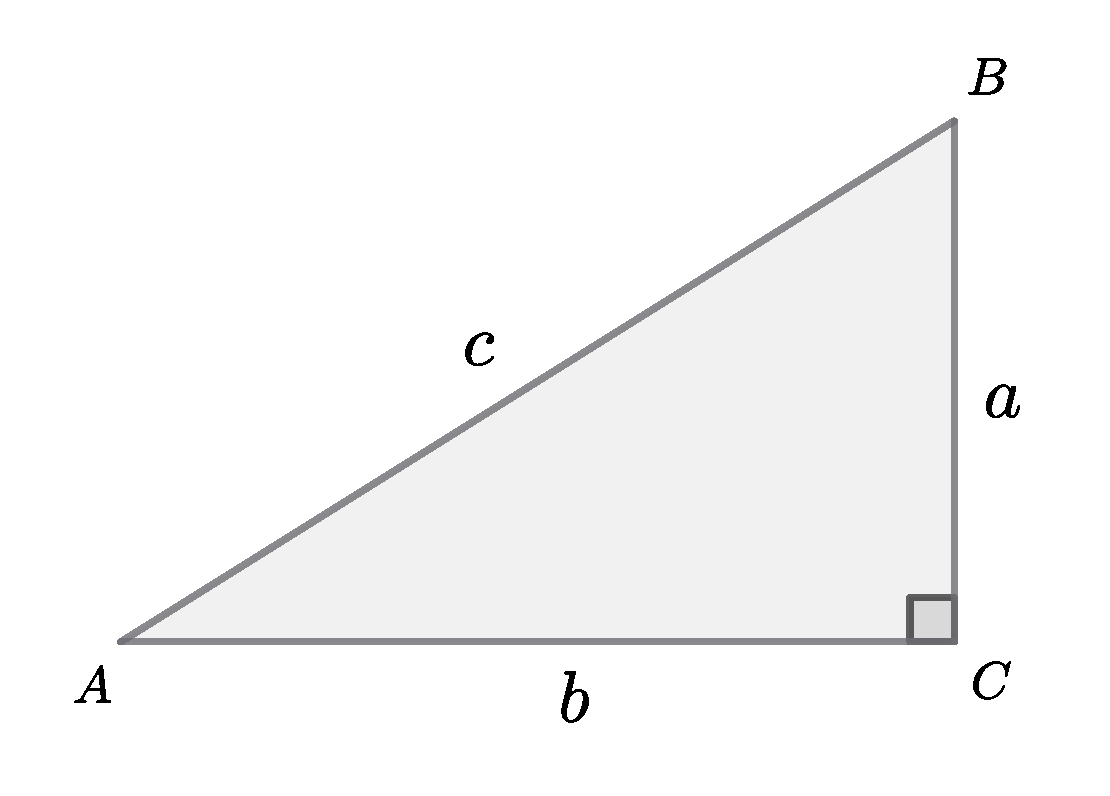
\includegraphics[scale=0.5]{50} 
\caption{} 
\label{Figure50} 
\end{figure}
\begin{itemize}
\item $AB$ เป็น \textbf{ด้านตรงข้ามมุมฉาก} (ด้านยาวที่สุดของสามเหลี่ยม) และมีความยาว $c$ หน่วย
\item $BC$ เป็น \textbf{ด้านตรงข้ามมุม} $A$ และมีความยาว $a$ หน่วย
\item $AC$ เป็น \textbf{ด้านตรงข้ามมุม} $B$ และมีความยาว $b$ หน่วย
\end{itemize}
จากรูปที่~\ref{Figure50} สามารถนิยามอัตราส่วนตรีโกณมิติที่สัมพันธ์กับด้านของสามเหลี่ยมมุมฉากได้ดังต่อไปนี้
\newpage
\begin{remarkbox}
\begin{enumerate}
    \item \textbf{ไซน์ของมุม $A$} แทนด้วยสัญลักษณ์ $\sin(A)$ นิยามโดย
    \[
    \sin(A)=\frac{\text{ความยาวด้านที่อยู่ตรงข้ามมุม } A}{\text{ความยาวด้านตรงข้ามมุมฉาก}}
    =\frac{a}{c}
    \]

    \item \textbf{โคไซน์ของมุม $A$} แทนด้วยสัญลักษณ์ $\cos(A)$ นิยามโดย
    \[
    \cos(A)=\frac{\text{ความยาวด้านประชิดมุม } A}{\text{ความยาวด้านตรงข้ามมุมฉาก}}
    =\frac{b}{c}
    \]

    \item \textbf{แทนเจนต์ของมุม $A$} แทนด้วยสัญลักษณ์ $\tan(A)$ นิยามโดย
    \[
    \tan(A)=\frac{\text{ความยาวด้านที่อยู่ตรงข้ามมุม } A}{\text{ความยาวด้านประชิดมุม } A}
    =\frac{a}{b}
    \]
\end{enumerate}
\end{remarkbox}
\begin{remarkbox}
นอกจากอัตราส่วนตรีโกณมิติพื้นฐานแล้ว ยังมีอัตราส่วนตรีโกณมิติส่วนกลับอีก $3$ อัตราส่วน ดังนี้
\begin{enumerate}
    \item \textbf{โคซีแคนต์ของมุม $A$} แทนด้วยสัญลักษณ์ $\cosec(A)$ ซึ่งเป็นส่วนกลับของ $\sin(A)$
    \[
    \cosec(A)=\frac{1}{\sin(A)} \quad \text{เมื่อ } \sin(A)\neq 0
    \]

    \item \textbf{ซีแคนต์ของมุม $A$} แทนด้วยสัญลักษณ์ $\sec(A)$ ซึ่งเป็นส่วนกลับของ $\cos(A)$
    \[
    \sec(A)=\frac{1}{\cos(A)} \quad \text{เมื่อ } \cos(A)\neq 0
    \]

    \item \textbf{โคแทนเจนต์ของมุม $A$} แทนด้วยสัญลักษณ์ $\cot(A)$ ซึ่งเป็นส่วนกลับของ $\tan(A)$
    \[
    \cot(A)=\frac{1}{\tan(A)} \quad \text{เมื่อ } \tan(A)\neq 0
    \]
\end{enumerate}
\end{remarkbox}


\begin{observationbox}
เนื่องจาก $\sin(A)=\dfrac{a}{c},\,\,\cos(A)=\dfrac{b}{c}$ และ $\tan(A)=\dfrac{a}{b}$\\
\vspace{0.5cm}\\
จะเห็นได้ว่า $\tan(A)=\dfrac{\sin(A)}{\cos(A)}$ และ $\cot(A)=\dfrac{\cos(A)}{\sin(A)}$    
\end{observationbox}

\begin{examplebox}
กำหนดให้ $\triangle ABC$ เป็นสามเหลี่ยมที่มีมุม $C$ เป็นมุมฉาก ถ้า $\cos(A)=\dfrac{3}{5}$ จงหาค่าของ $\sin(A)$ และ $\tan(A)$
\end{examplebox}
\vspace{5cm}
\begin{examplebox}
กำหนดให้ $\triangle ABC$ เป็นสามเหลี่ยมที่มีมุม $C$ เป็นมุมฉาก ถ้า $\tan(A)=\dfrac{5}{12}$ จงหาค่าของ 
\[\dfrac{2\sin(A)+3\cos(A)}{\sin(A)-\cos(A)}\]
\end{examplebox}
\vspace{6cm}
\subsection{ค่าฟังก์ชันตรีโกณมิติของมุมพื้นฐาน}
ตารางต่อไปนี้แสดงค่าฟังก์ชันตรีโกณมิติของมุมพื้นฐานที่ใช้บ่อย ในหน่วยองศา
\begin{table}[h]
\centering
\setlength{\extrarowheight}{4pt}
\begin{tabular}{|c|c|c|c|c|c|c|c|c|}
\hline
$\theta\,(\text{องศา})$ 
& $0^\circ$ 
& $30^\circ$ 
& $45^\circ$ 
& $60^\circ$ 
& $90^\circ$ 
& $180^\circ$
& $270^\circ$
& $360^\circ$\\
\hline

$\sin(\theta)$ 
& $0$ 
& $\dfrac{1}{2}$ 
& $\dfrac{\sqrt{2}}{2}$ 
& $\dfrac{\sqrt{3}}{2}$ 
& $1$ 
& $0$ 
& $-1$ 
& $0$ \\ 
\hline

$\cos(\theta)$ 
& $1$ 
& $\dfrac{\sqrt{3}}{2}$ 
& $\dfrac{\sqrt{2}}{2}$ 
& $\dfrac{1}{2}$ 
& $0$ 
& $-1$ 
& $0$ 
& $1$ \\
\hline

$\tan(\theta)$ 
& $0$ 
& $\dfrac{1}{\sqrt{3}}$ 
& $1$ 
& $\sqrt{3}$ 
& \text{ไม่กำหนดค่า}
& $0$ 
& \text{ไม่กำหนดค่า} 
& $0$ \\
\hline
\end{tabular}
\caption{ค่าฟังก์ชันตรีโกณมิติของมุมพื้นฐานในหน่วยองศา}
\label{table1.1}
\end{table}

\newpage
\section{องศาและเรเดียน}
หน่วยวัดขนาดของมุมที่ใช้กันทั่วไปมี $2$ หน่วย คือ \textbf{องศา} และ \textbf{เรเดียน} 
โดยสามารถแปลงหน่วยระหว่างกันได้ดังนี้
\begin{conceptbox}
 \begin{itemize}
    \item[*] การแปลงจาก \textbf{เรเดียน} เป็น \textbf{องศา} ให้แทน $\pi$ ด้วย $180^\circ$
    \item[*] การแปลงจาก \textbf{องศา} เป็น \textbf{เรเดียน} ให้คูณด้วย $\dfrac{\pi}{180}$
\end{itemize}   
\end{conceptbox}

\begin{examplebox}[NETSAT คณิตศาสตร์ กุมภาพันธ์ 2567]  
$72^{\circ}$ เท่ากับกี่เรเดียน
\begin{multicols}{2}
\begin{enumerate}
\item $\dfrac{2\pi}{3}$
\item $\dfrac{2\pi}{5}$
\item $\dfrac{3\pi}{4}$
\item $\dfrac{3\pi}{5}$
\end{enumerate}
  \end{multicols}
\end{examplebox}

\begin{examplebox}
จงเปลี่ยนมุมพื้นฐานต่อไปนี้ให้อยู่ในหน่วยเรเดียน
\begin{enumerate}
\item $0^\circ$ 
\item $30^\circ$ 
\item $45^\circ$ 
\item $60^\circ$ 
\item $90^\circ$ 
\item $180^\circ$
\item $270^\circ$
\item $360^\circ$
\end{enumerate}
\end{examplebox}

จากตารางที่~\ref{table1.1} สามารถเขียนค่าฟังก์ชันตรีโกณมิติของมุมพื้นฐานในหน่วยเรเดียนได้ดังตารางต่อไปนี้

\begin{table}[h]
\centering
\setlength{\extrarowheight}{4pt}
\begin{tabular}{|c|c|c|c|c|c|c|c|c|}
\hline
$\theta\,(\text{เรเดียน})$ 
& $0$ 
& $\dfrac{\pi}{6}$ 
& $\dfrac{\pi}{4}$ 
& $\dfrac{\pi}{3}$ 
& $\dfrac{\pi}{2}$ 
& $\pi$ 
& $\dfrac{3\pi}{2}$ 
& $2\pi$ \\
\hline

$\sin(\theta)$ 
& $0$ 
& $\dfrac{1}{2}$ 
& $\dfrac{\sqrt{2}}{2}$ 
& $\dfrac{\sqrt{3}}{2}$ 
& $1$ 
& $0$ 
& $-1$ 
& $0$ \\ 
\hline

$\cos(\theta)$ 
& $1$ 
& $\dfrac{\sqrt{3}}{2}$ 
& $\dfrac{\sqrt{2}}{2}$ 
& $\dfrac{1}{2}$ 
& $0$ 
& $-1$ 
& $0$ 
& $1$ \\
\hline

$\tan(\theta)$ 
& $0$ 
& $\dfrac{1}{\sqrt{3}}$ 
& $1$ 
& $\sqrt{3}$ 
& \text{ไม่กำหนดค่า}
& $0$ 
& \text{ไม่กำหนดค่า} 
& $0$ \\
\hline
\end{tabular}
\caption{ค่าฟังก์ชันตรีโกณมิติของมุมพื้นฐานในหน่วยเรเดียน}
\label{table1.2}
\end{table}


\section{ทบทวนสูตรตรีโกณมิติที่จำเป็น}
\subsection{โคฟังก์ชัน}
สำหรับ $0^{\circ}<\theta<90^{\circ}$ จะมีความสัมพันธ์ของโคฟังก์ชันดังนี้
\begin{itemize}
\item $\sin(\theta)=\cos\left(90^\circ-\theta\right)$
\item $\tan(\theta)=\cot\left(90^\circ-\theta\right)$
\item $\sec(\theta)=\cosec\left(90^\circ-\theta\right)$
\end{itemize}

\subsection{เอกลักษณ์ตรีโกณมิติ}
เอกลักษณ์ตรีโกณมิติพื้นฐานที่ใช้บ่อย มีดังนี้
\begin{itemize}
\item $\sin^2(\theta)+\cos^2(\theta)=1$ 
\item $\sec^2(\theta)-\tan^2(\theta)=1$ 
\item $\cosec^2(\theta)-\cot^2(\theta)=1$ 
\end{itemize}

\subsection{ฟังก์ชันตรีโกณมิติของมุมสองเท่า}
ถ้า $\alpha$ เป็นจำนวนจริง จะมีสูตรมุมสองเท่าดังนี้
\begin{itemize}
\item $\sin(2\alpha)=2\sin(\alpha)\cos(\alpha)$
\item $\cos(2\alpha)=\cos^2(\alpha)-\sin^2(\alpha)$
\end{itemize}

\subsection{ฟังก์ชันตรีโกณมิติของผลบวกและผลต่างของมุม}
ให้ $A$ และ $B$ เป็นจำนวนจริง จะได้ว่า
\begin{itemize}
\item $\sin(A+B)=\sin(A)\cos(B)+\cos(A)\sin(B)$ 
\item $\sin(A-B)=\sin(A)\cos(B)-\cos(A)\sin(B)$ 
\item $\cos(A+B)=\cos(A)\cos(B)-\sin(A)\sin(B)$ 
\item $\cos(A-B)=\cos(A)\cos(B)+\sin(A)\sin(B)$
\item $\tan(A+B)=\dfrac{\tan(A)+\tan(B)}{1-\tan(A)\tan(B)}$  
\item $\tan(A-B)=\dfrac{\tan(A)-\tan(B)}{1+\tan(A)\tan(B)}$ 
\end{itemize}

\begin{remarkbox}\label{remark1.3}
สำหรับจำนวนจริง $\theta$ จะมีสมบัติดังนี้
\begin{itemize}
\item $\sin(-\theta)=-\sin(\theta)$
\item $\cos(-\theta)=\cos(\theta)$
\item $\tan(-\theta)=-\tan(\theta)$
\end{itemize}
\end{remarkbox}

\begin{observationbox}\label{observation1.2}
 \begin{enumerate}
     \item $\sin(30^{\circ})=\dfrac{1}{2}$
     \item $\sin\left(\dfrac{\pi}{6}\right)=\dfrac{1}{2}$
 \end{enumerate}
\end{observationbox}
เมื่อมุมมีขนาดมากกว่า $90^{\circ}$ หรือมีค่ามากกว่า $\frac{\pi}{2}$ การหาค่าฟังก์ชันตรีโกณมิติจะไม่สามารถอาศัยตารางมุมพิเศษโดยตรงได้ จึงจำเป็นต้องยุบมุมให้อยู่ในช่วงที่คุ้นเคยก่อน

\begin{observationbox}\label{observation1.3}
 \begin{enumerate}
     \item $\sin(210^{\circ})=?$
     \item $\sin\left(\dfrac{7\pi}{6}\right)=?$
 \end{enumerate}
\end{observationbox}
\newpage
\section{การแปลงมุมในรูปอย่างง่าย}
\subsection{เครื่องหมายและจตุภาค (ควอดรันท์)} \label{section1.4.1}
จากรูปที่~\ref{Figure51} สัญลักษณ์ $Q_1,Q_2,Q_3$ และ $Q_4$ หมายถึง
\textbf{จตุภาคที่หนึ่ง จตุภาคที่สอง จตุภาคที่สาม และจตุภาคที่สี่}
(หรือเรียกว่า \textbf{ควอดรันท์ที่หนึ่ง สอง สาม และสี่}) ตามลำดับ
เราจะได้เครื่องหมายของฟังก์ชันตรีโกณมิติ $\sin$ และ $\cos$
ในแต่ละจตุภาคดังต่อไปนี้

\begin{figure}[H]	 
	\centering
	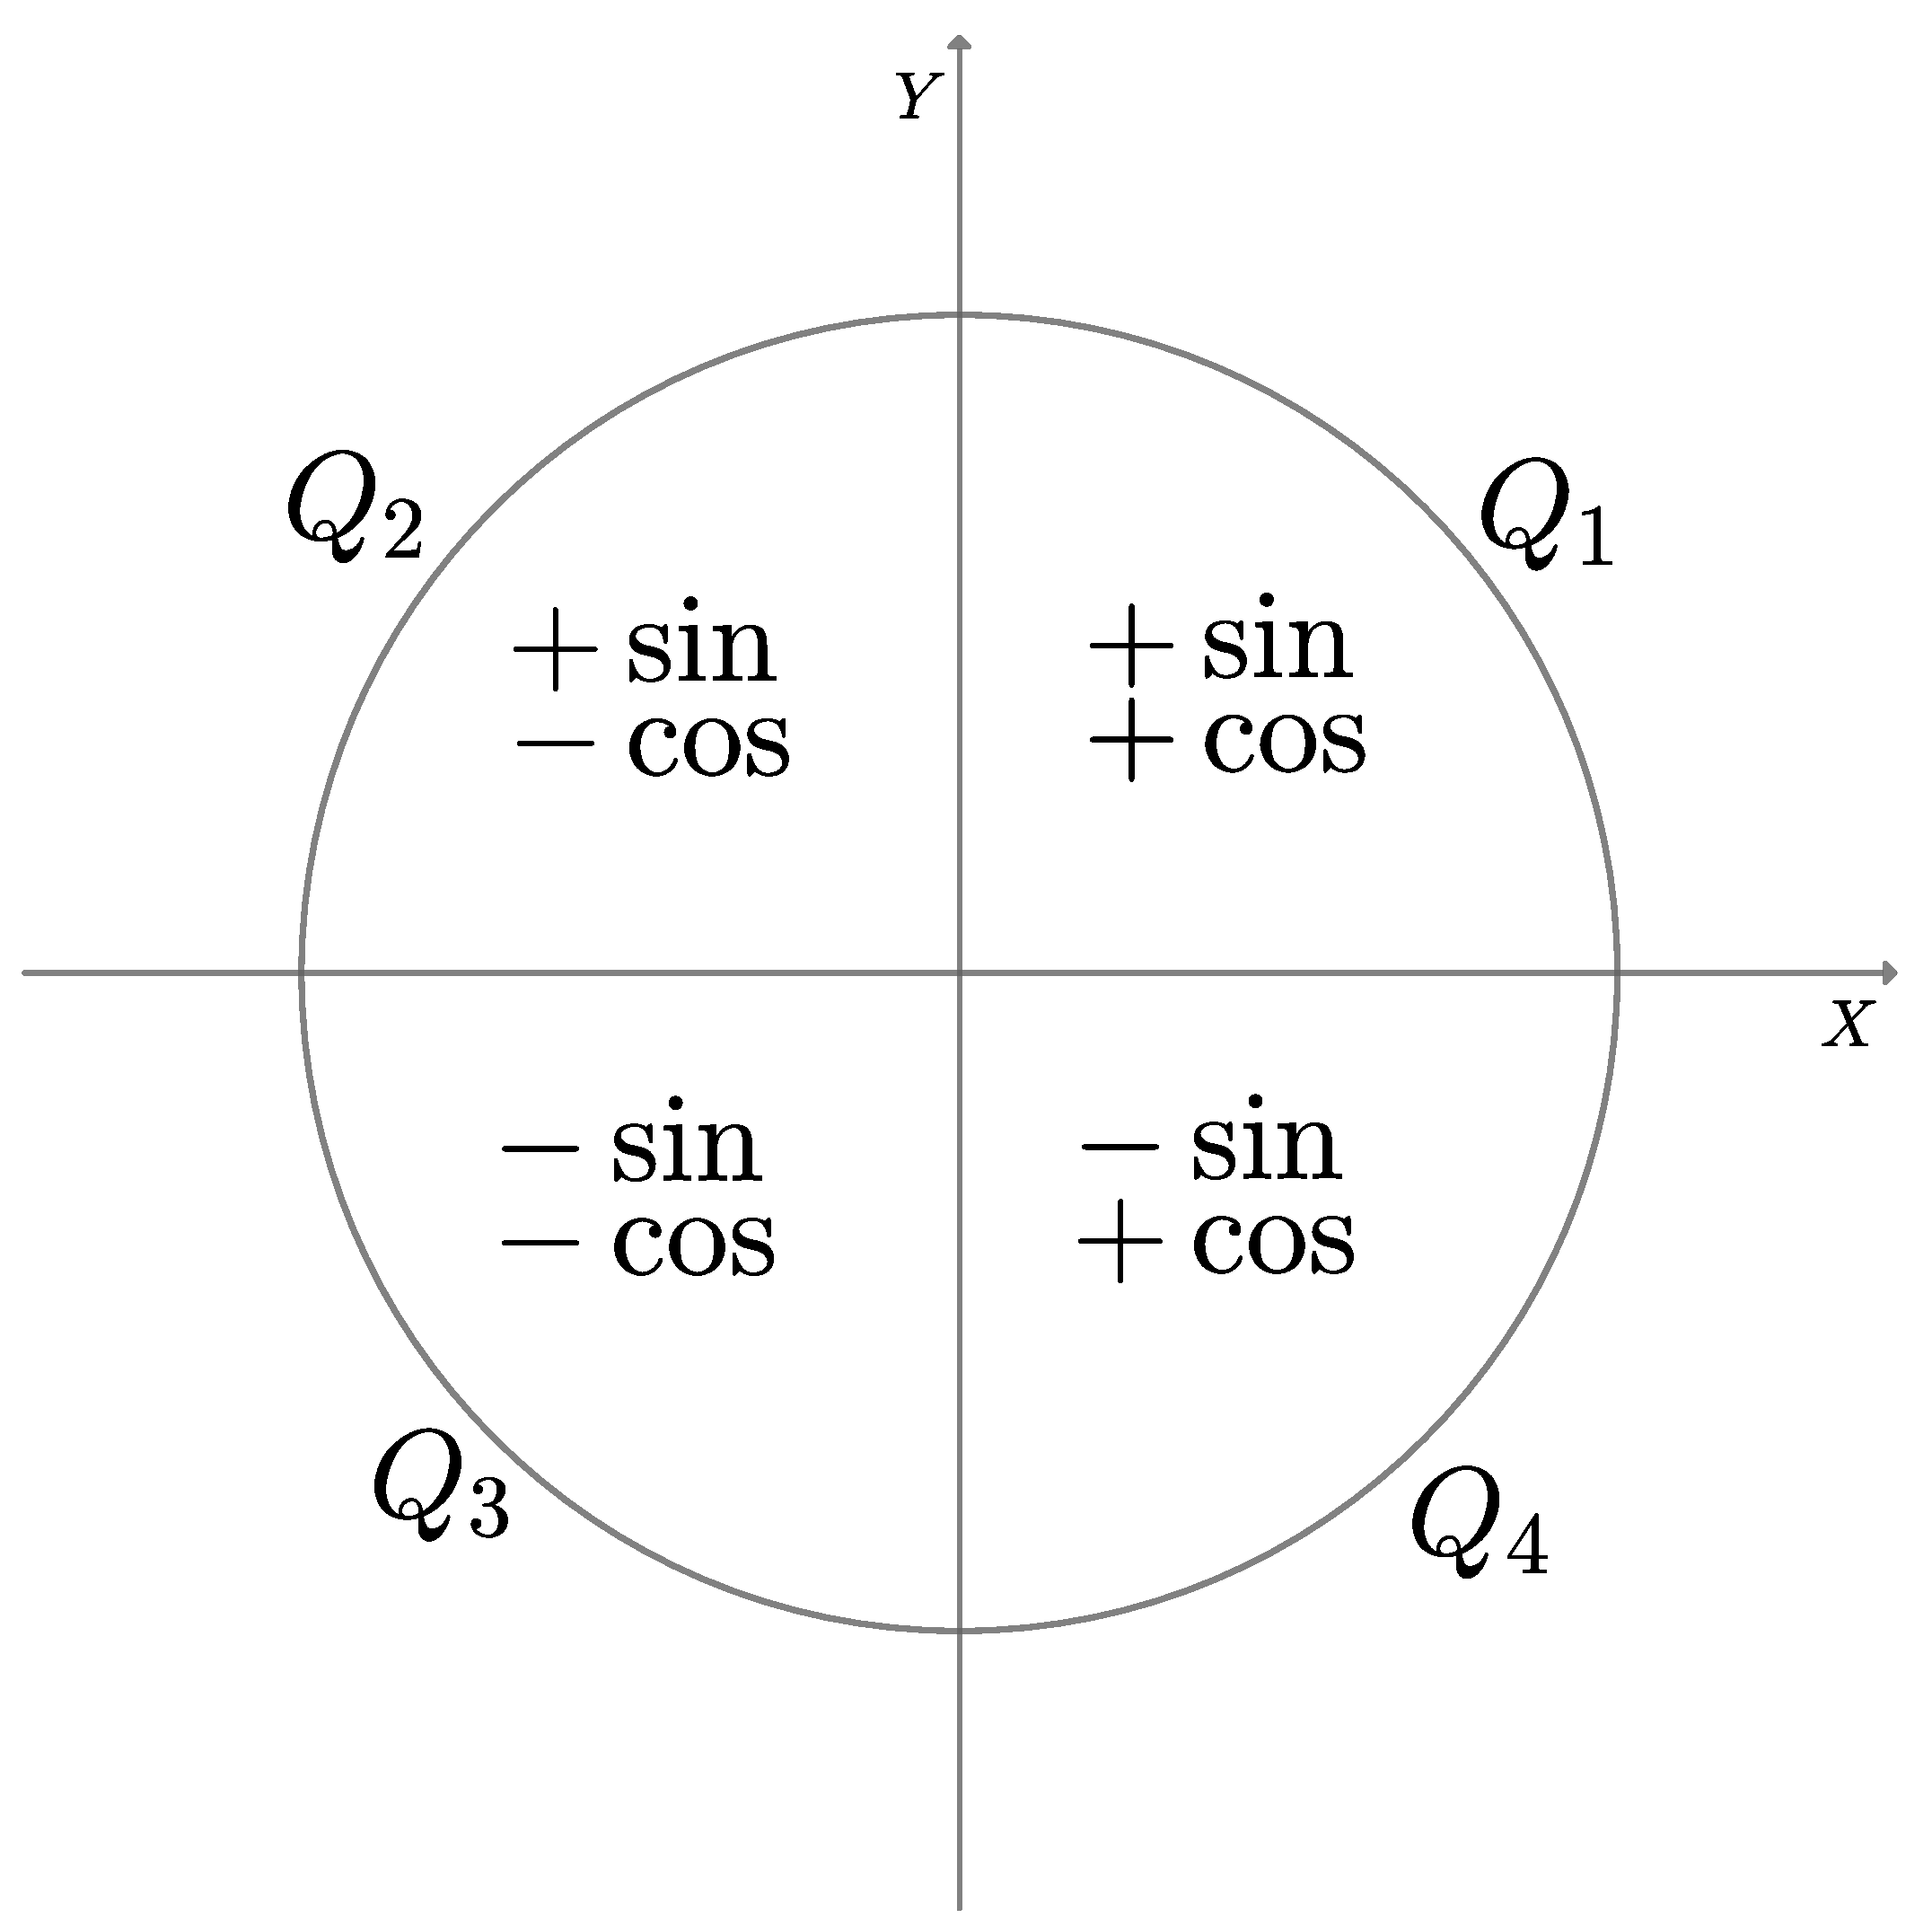
\includegraphics[scale=0.5]{52}
    	\caption{}
       \label{Figure52}
\end{figure} 
\newpage

\begin{examplebox}
ถ้า $\sin(\theta)>0$ และ $\cos(\theta)<0$ แล้ว $\theta$ อยู่ควอดรันท์ใด
\end{examplebox}
\vspace{8cm}

\begin{examplebox}
กำหนดให้ $\tan^2(\theta)=\dfrac{1}{5}$ และ $\theta$ อยู่ควอดรันท์ที่สอง จงหาค่า $\cot(\theta)$
\end{examplebox}

\newpage
\subsection{การวัดมุม}
\begin{figure}[H]	 
	\centering
	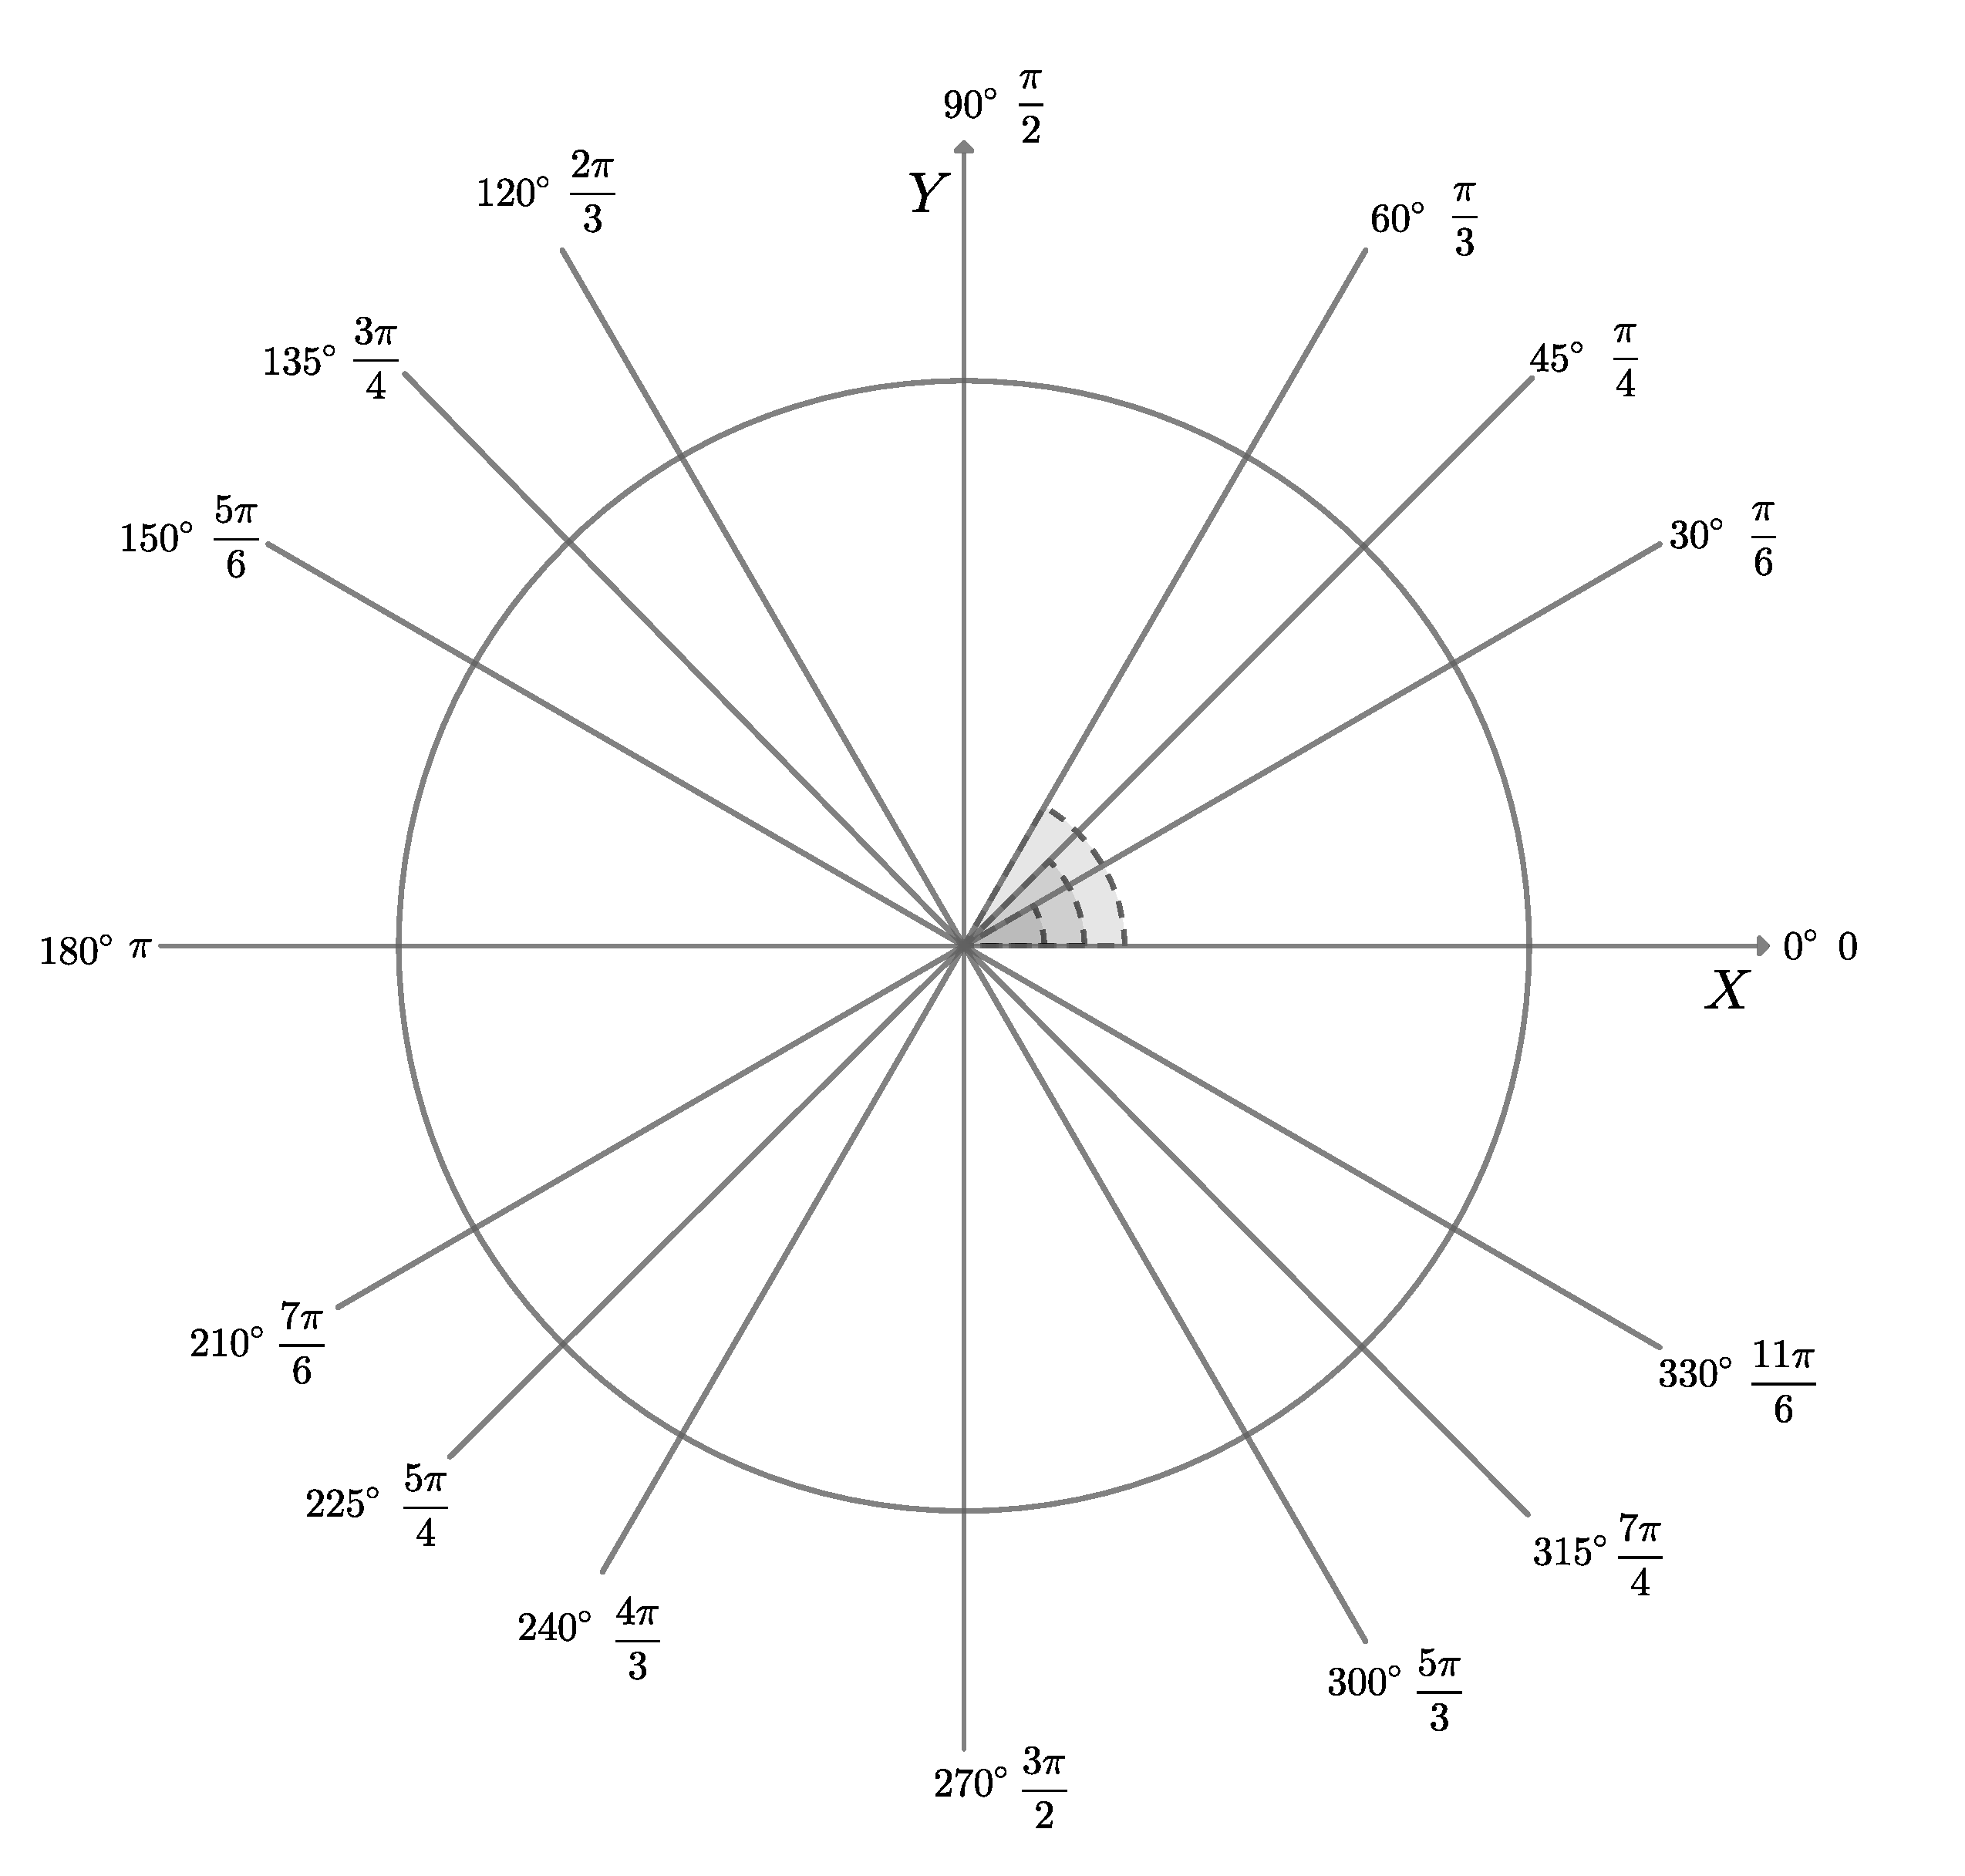
\includegraphics[scale=0.48]{51}
    	\caption{}
       \label{Figure51}
\end{figure} 
\newpage
\begin{examplebox}[NETSAT คณิตศาสตร์ สิงหาคม 2568]
กำหนดให้ $0<A<\dfrac{\pi}{2}$ และ $\tan(A)=2.4$ จงหาค่า $\cos(A)$
\begin{multicols}{2}
\begin{enumerate}
\item $\dfrac{5}{12}$
\item $\dfrac{5}{13}$
\item $-\dfrac{5}{12}$
\item $-\dfrac{5}{13}$
\end{enumerate}
\end{multicols}
\end{examplebox}
\newpage
\subsection{มุมคู่ $\pi$ และมุมคี่ $\pi$}
จากรูปที่~\ref{Figure53} สามารถจำแนกมุมที่เป็นพหุคูณของ $\pi$ ได้ดังนี้
\begin{itemize}
    \item \textbf{มุมคู่ $\pi$} คือ มุมที่สามารถเขียนได้ในรูป $2n\pi$ เมื่อ $n$ เป็นจำนวนเต็มไม่ลบ กล่าวคือ $n=0,1,2,\ldots$
    \item \textbf{มุมคี่ $\pi$} คือ มุมที่สามารถเขียนได้ในรูป $(2n+1)\pi$ เมื่อ $n$ เป็นจำนวนเต็มไม่ลบ กล่าวคือ $n=0,1,2,\ldots$
\end{itemize}
\begin{figure}[H]	 
	\centering
	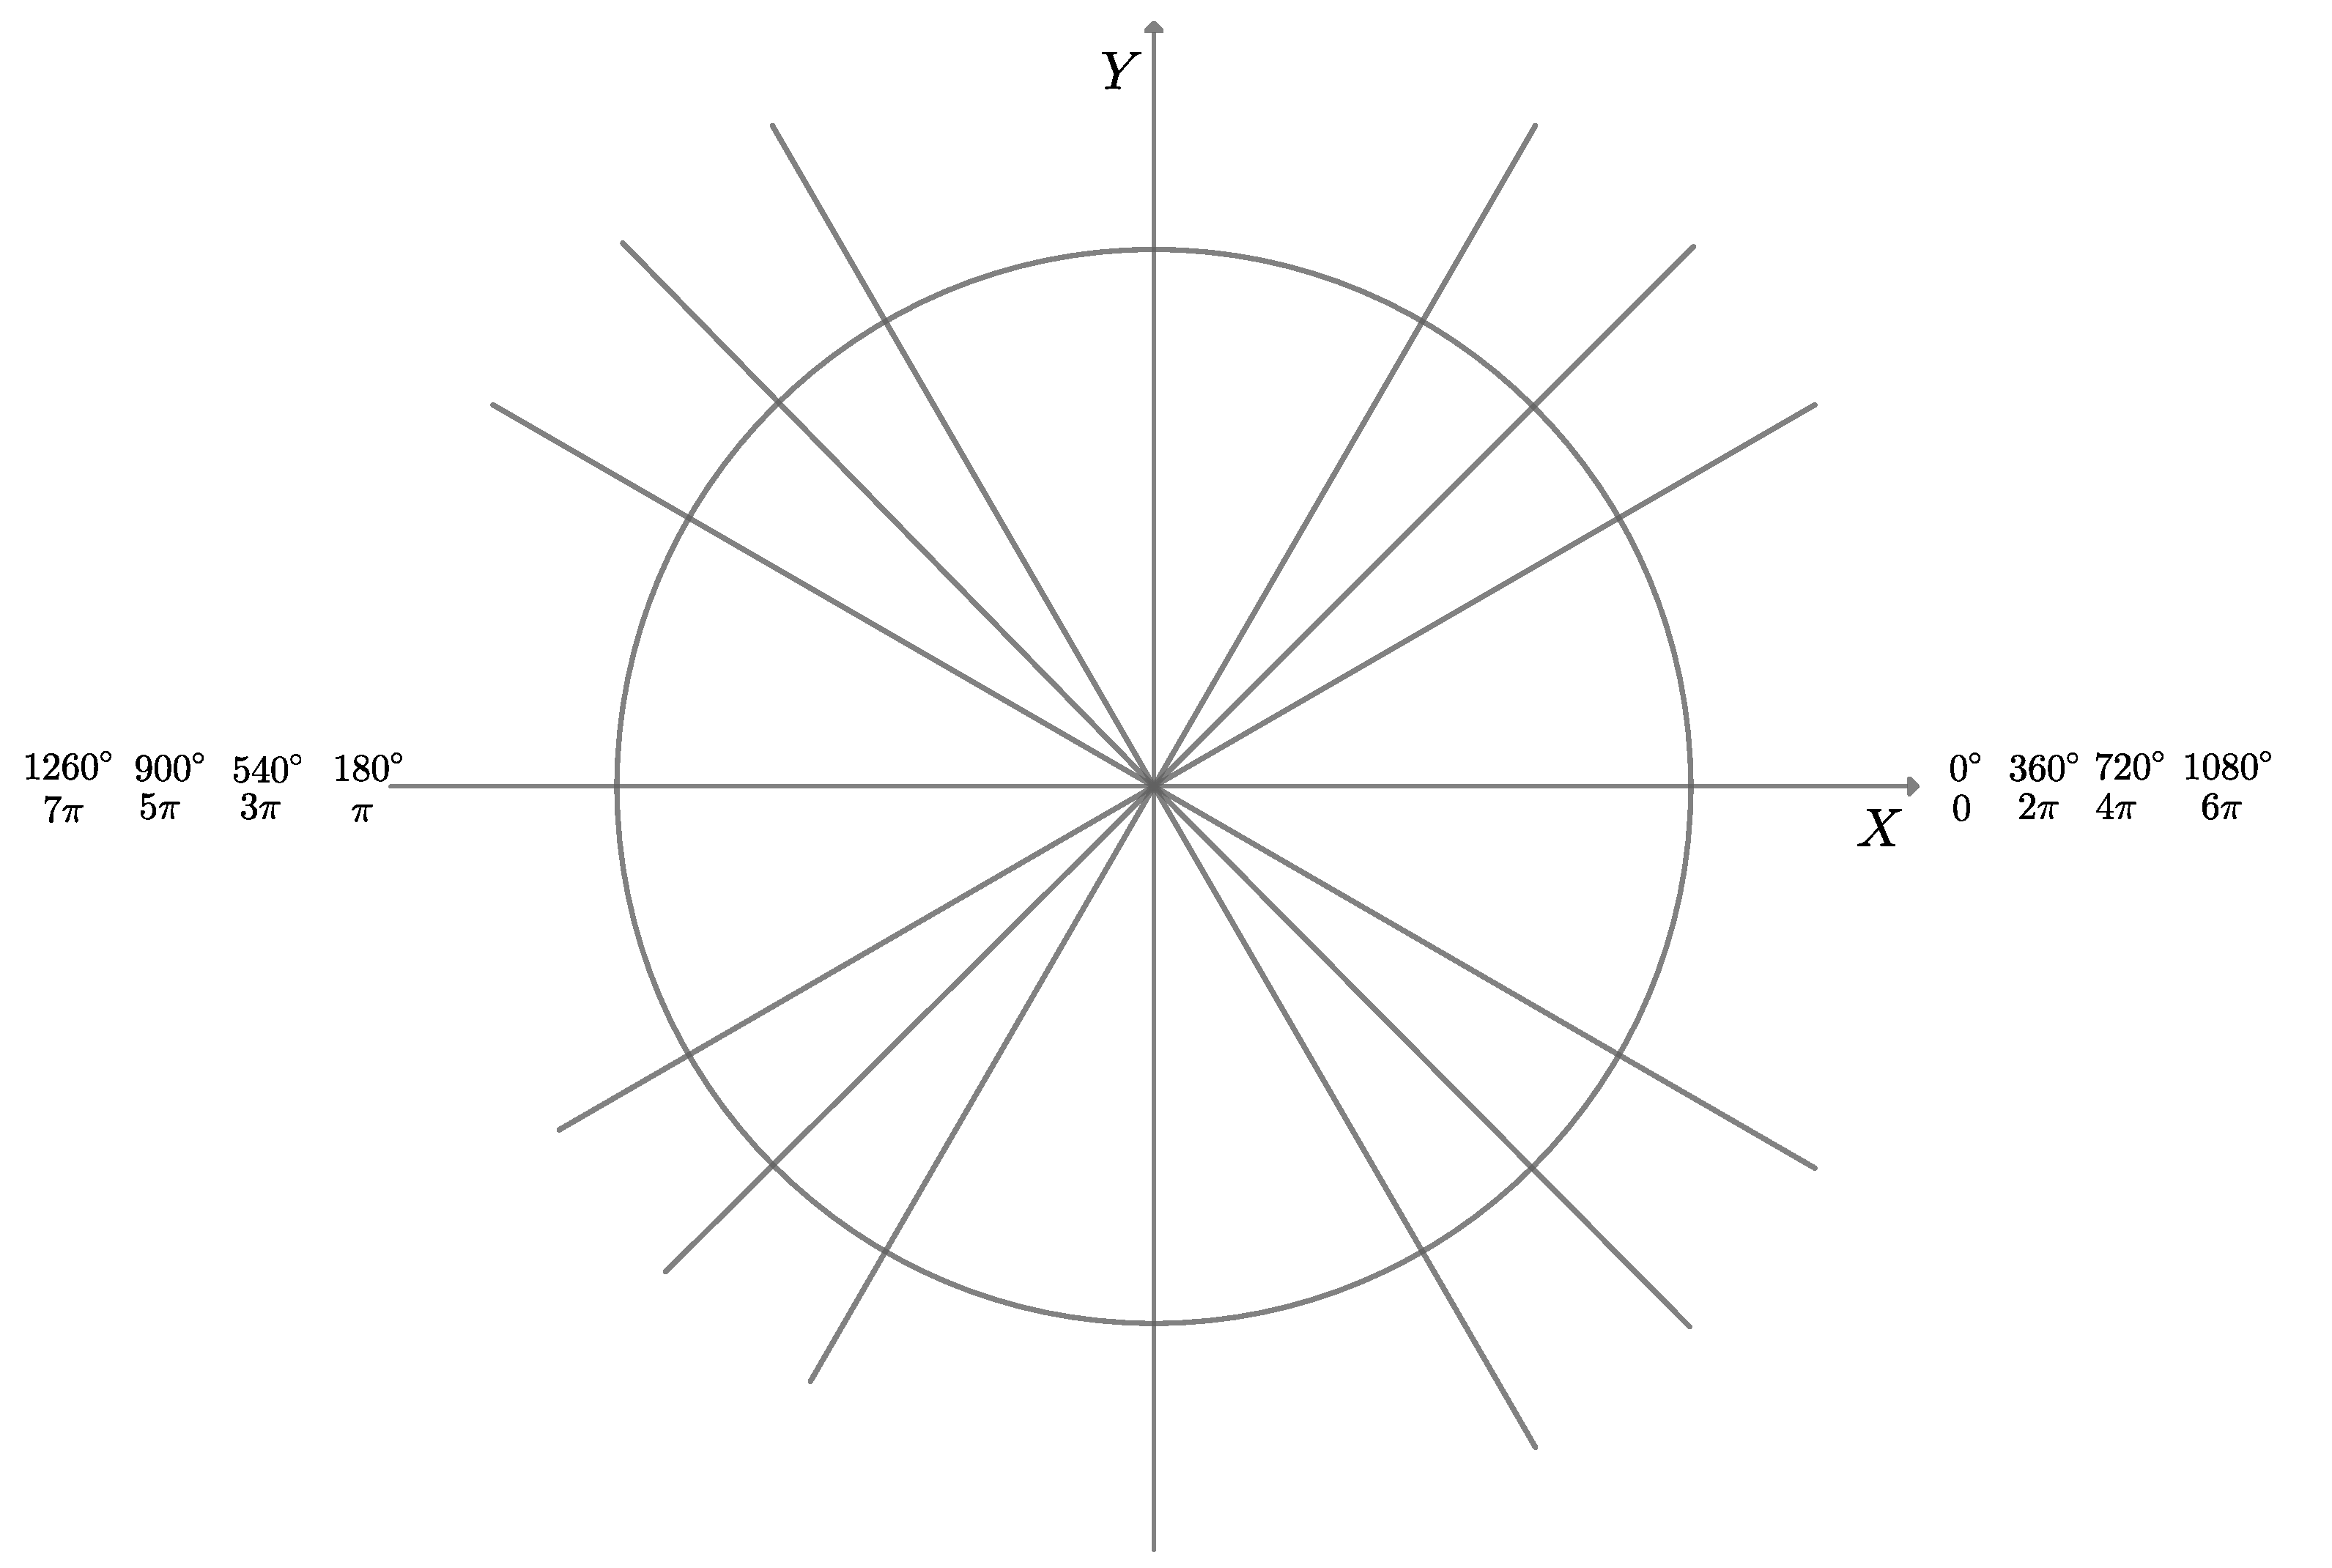
\includegraphics[scale=0.37]{53}
    	\caption{}
       \label{Figure53}
\end{figure} 

\newpage
\subsection{ค่าฟังก์ชันตรีโกณมิติของมุมเรเดียนในรูป $2n\pi \pm \theta$ และ $(2n+1)\pi \pm \theta$ 
เมื่อ $n$ เป็นจำนวนเต็มไม่ลบ}

\begin{conceptbox}\label{concept5.2}
ให้ $\alpha$ เป็นมุมในหน่วยเรเดียน สามารถหาค่าฟังก์ชันตรีโกณมิติของมุม $\alpha$ ได้ตามขั้นตอนดังนี้
\begin{enumerate}
    \item พิจารณาเครื่องหมายของมุม $\alpha$
    \begin{enumerate}[label*=\arabic*.]
        \item หาก $\alpha>0$ ให้ดำเนินการตามข้อ 2
        \item หาก $\alpha<0$ ให้ใช้สมบัติของฟังก์ชันตรีโกณมิติของมุมลบ 
        (ดูข้อควรรู้~\ref{remark1.3}) เพื่อแปลงเป็นมุมบวกก่อน แล้วจึงดำเนินการตามข้อ 2
    \end{enumerate}
    \item เขียนมุม $\alpha$ ให้อยู่ในรูป  
    \[
    2n\pi \pm \theta \quad \text{หรือ} \quad (2n+1)\pi \pm \theta
    \]
    เมื่อ $n$ เป็นจำนวนเต็มไม่ลบ และ $0<\theta<\dfrac{\pi}{2}$
    \item ตรวจสอบว่ามุมที่ได้อยู่ในควอดรันท์ใด
    \item ค่าฟังก์ชันตรีโกณมิติของมุม $\alpha$ จะเท่ากับ
    ค่าฟังก์ชันตรีโกณมิติของมุม $\theta$ 
    โดยพิจารณาเครื่องหมายของฟังก์ชันตามควอดรันท์นั้น
    (ตามที่กล่าวไว้ในหัวข้อย่อย~\ref{section1.4.1})
\end{enumerate}
\end{conceptbox}

\begin{examplebox}
จงหาค่าฟังก์ชันตรีโกณมิติต่อไปนี้ เมื่อกำหนดให้ $0<\theta<\dfrac{\pi}{2}$
\begin{enumerate}
    \item $\sin(3\pi+\theta)$  

    เนื่องจาก $3\pi+\theta$ อยู่ในควอดรันท์ที่ 3  
    \[
    \sin(3\pi+\theta)=-\sin(\theta)
    \]

    \item $\cos(2\pi+\theta)$  

    เนื่องจาก $2\pi+\theta$ อยู่ในควอดรันท์ที่ 1  
    \[
    \cos(2\pi+\theta)=\cos(\theta)
    \]

    \item $\tan(5\pi-\theta)$  

    เนื่องจาก $5\pi-\theta$ อยู่ในควอดรันท์ที่ 2  
    \[
    \tan(5\pi-\theta)=-\tan(\theta)
    \]
    
    \item $\cosec(10\pi-\theta)$  

    เนื่องจาก $10\pi-\theta$ อยู่ในควอดรันท์ที่ 4  
    \[
    \cosec(10\pi-\theta)=-\cosec(\theta)
    \]
\end{enumerate}
\end{examplebox}

\begin{examplebox}
จงหาค่าฟังก์ชันตรีโกณมิติต่อไปนี้ เมื่อกำหนดให้ $0<\theta<\dfrac{\pi}{2}$
\begin{enumerate}
    \item $\cot(\theta-\pi)$  
   \[
    \cot(\theta-\pi)
    =-\cot(\pi-\theta)
    \]
เนื่องจาก $\pi-\theta$ อยู่ในควอดรันท์ที่ 2 ดังนั้น $\cot(\pi-\theta)=-\cot(\theta)$\\
จึงได้ว่า
  \[
    \cot(\theta-\pi)
    =-(-\cot(\theta))
    =\cot(\theta)
    \]
    \item $\sec(-2\pi-\theta)$  
    \[
    \sec(-2\pi-\theta)
    =\sec(2\pi+\theta)
    \]
เนื่องจาก $2\pi+\theta$ อยู่ในควอดรันท์ที่ 1 ดังนั้น    
    \[
    \sec(-2\pi-\theta)
    =\sec(2\pi+\theta)
    =\sec(\theta)
    \]
\end{enumerate}
\end{examplebox}

\begin{examplebox}
จงหาค่าของ $\sin\left(\dfrac{8\pi}{3}\right)$
\end{examplebox}
\vspace{3cm}
\begin{examplebox}
จงหาค่าของ $\sin\left(-\dfrac{7\pi}{6}\right)$
\end{examplebox}
\vspace{3cm}
\begin{examplebox}
จงหาค่าของ $\cos\left(\dfrac{8\pi}{3}\right)$
\end{examplebox}
\vspace{3cm}
\begin{examplebox}
จงหาค่าของ $\cos\left(-\dfrac{11\pi}{3}\right)$
\end{examplebox}
\vspace{3cm}
\begin{examplebox}
จงหาค่าของ $\tan\left(\dfrac{4\pi}{3}\right)$
\end{examplebox}
\vspace{3cm}
\begin{examplebox}
จงหาค่าของ $\cosec\left(\dfrac{13\pi}{6}\right)$
\end{examplebox}
\vspace{3cm}
\begin{examplebox}
จงหาค่าของ $\tan\left(-\dfrac{13\pi}{6}\right)$
\end{examplebox}
\newpage
\begin{examplebox}
จงหาค่าของ $\cot\left(\dfrac{9\pi}{5}\right)$
\end{examplebox}
\vspace{3cm}
\begin{examplebox}
จงหาค่าของ 
\[\dfrac{\sin\left(\dfrac{3\pi}{8} \right)}{\sin\left(\dfrac{5\pi}{8} \right)}+ \dfrac{\tan\left(\dfrac{13\pi}{7}\right)}{\tan\left(\dfrac{\pi}{7} \right)}\]
\end{examplebox}
\newpage
\begin{observationbox}
จากหลักการ~\ref{concept5.2} เราสามารถประยุกต์ใช้เพื่อหาค่าฟังก์ชันตรีโกณมิติของมุมในหน่วยองศาได้ โดยมีแนวคิดเช่นเดียวกัน กล่าวคือ
ให้ $\alpha>0$ เป็นมุมในหน่วยองศา สามารถเขียนมุม $\alpha$ ให้อยู่ในรูป
\[
\left(n\times 180^{\circ}\right)\pm\theta
\]
เมื่อ $n$ เป็นจำนวนเต็มไม่ลบ กล่าวคือ $n=0,1,2,\ldots$ และ $0^{\circ}<\theta<90^{\circ}$
จากนั้นพิจารณาควอดรันท์ของมุมที่ได้ และกำหนดเครื่องหมายของฟังก์ชันตรีโกณมิติตามควอดรันท์นั้น โดยค่าฟังก์ชันตรีโกณมิติของมุม $\alpha$ จะเท่ากับค่าฟังก์ชันตรีโกณมิติของมุม $\theta$
\end{observationbox}


\begin{examplebox}
จงหาค่าของ $\cosec\left(150^{\circ}\right)$
\end{examplebox}
\vspace{3cm}
\begin{examplebox}
จงหาค่าของ $\sec\left(-315^{\circ}\right)$
\end{examplebox}
\vspace{3cm}
\begin{examplebox}
จงหาค่าของ $\cot\left(-1020^{\circ}\right)$
\end{examplebox}
\vspace{3cm}
\begin{examplebox}
จงหาค่าของ $\sin\left(210^{\circ}\right)$
\end{examplebox}
\newpage
\begin{examplebox}
จงหาค่าของ $\tan\left(-585^{\circ}\right)$
\end{examplebox}
\vspace{3cm}
\begin{examplebox}
จงหาค่าของ $\cos\left(765^{\circ}\right)$
\end{examplebox}
\vspace{3cm}
\begin{examplebox}
จงหาค่าของ 
\[\dfrac{\sin(-420^{\circ})\cot(210^{{\circ}})+\sqrt{3}\cot(-390^{{\circ}})-1}{\cos(-840^{\circ})}\]
\end{examplebox}
\newpage
\begin{examplebox}[NETSAT คณิตศาสตร์ สิงหาคม 2565]
ถ้า $A$ อยู่ในจตุภาคที่ 1 โดยที่ $0^{\circ}<A<90^{\circ}$ แล้ว $\cos(90^{\circ}-A)$ มีค่าเท่ากับเท่าใด
\begin{multicols}{2}
\begin{enumerate}
\item $\sin(A)$
\item $\cos(A)$
\item $-\sin(A)$
\item $-\cos(A)$
\end{enumerate}
\end{multicols}
\end{examplebox}
\newpage
\begin{examplebox}[NETSAT คณิตศาสตร์ สิงหาคม 2565]
กำหนด $0^{\circ}<A<90^{\circ}$ จงหาค่าของ 
\[\sin(90^{\circ}-A)\cos(A)\tan^2(A)+\dfrac{\sin(A) \cos(90^{\circ}-A)}{\tan^2(A)}\]
\begin{multicols}{2}
\begin{enumerate}
\item $-1$
\item $1$
\item $\sin(2A)$
\item $\cos(2A)$
\end{enumerate}
\end{multicols}
\end{examplebox}
\newpage
\begin{examplebox}[NETSAT คณิตศาสตร์ กุมภาพันธ์ 2565]
ถ้า $\tan(\theta)=-10$ เมื่อ $90^{\circ}<\theta<180^{\circ}$ แล้ว $\cos(\theta)$ มีค่าเท่าใด
\begin{multicols}{2}
\begin{enumerate}
\item $\dfrac{-1}{\sqrt{101}}$
\item $\dfrac{1}{\sqrt{101}}$
\item $\dfrac{10}{\sqrt{101}}$
\item $\dfrac{-10}{\sqrt{101}}$
\end{enumerate}
\end{multicols}
\end{examplebox}
\newpage
\begin{examplebox}[NETSAT คณิตศาสตร์ กุมภาพันธ์ 2565]
ถ้า $\theta$ เป็นมุม ซึ่ง $270^{\circ}<\theta<360^{\circ}$ และ $\sin(\theta)=-\dfrac{1}{4}$ แล้ว $\sin(2\theta)$ มีค่าเท่าใด
\begin{multicols}{2}
\begin{enumerate}
\item $-\dfrac{\sqrt{15}}{8}$
\item $\dfrac{\sqrt{15}}{8}$
\item $-\dfrac{\sqrt{15}}{4}$
\item $\dfrac{\sqrt{15}}{4}$
\end{enumerate}
\end{multicols}
\end{examplebox}

\newpage
\begin{examplebox}[NETSAT คณิตศาสตร์ สิงหาคม 2565]
ถ้า $\tan(\theta)=3$ สำหรับ $0^{\circ}<\theta<90^{\circ}$ แล้ว $\cos(\theta)+\sin( \theta)$ มีค่าเท่าใด
\begin{multicols}{2}
\begin{enumerate}
\item $\dfrac{1}{\sqrt{10}}$
\item $\dfrac{2}{\sqrt{10}}$
\item $\dfrac{3}{\sqrt{10}}$
\item $\dfrac{4}{\sqrt{10}}$
\end{enumerate}
\end{multicols}
\end{examplebox}
\newpage
\begin{examplebox}[NETSAT คณิตศาสตร์ สิงหาคม 2566]
ให้ $\theta=135^{\circ}$ และ $x=\cos(\theta), y=\sin(\theta)$ แล้ว $x-y$ มีค่าเท่าใด
\begin{multicols}{2}
\begin{enumerate}
\item $-\sqrt{2}$
\item $0$
\item $1$
\item $\sqrt{2}$
\end{enumerate}
\end{multicols}
\end{examplebox}
\newpage
\section{กฎของโคไซน์และกฎของไซน์}
\begin{theorembox}[กฎของโคไซน์]
กำหนดให้ $\triangle ABC$ เป็นสามเหลี่ยมใด ๆ
ซึ่งมีความยาวด้านตรงข้ามมุม $A,B$ และ $C$
เท่ากับ $a,b$ และ $c$ ตามลำดับ ดังรูปที่~\ref{Figure25}
จะได้ความสัมพันธ์ดังต่อไปนี้
\begin{align*}
a^2 &= b^2+c^2-2bc\cos(A)\\
b^2 &= c^2+a^2-2ca\cos(B)\\
c^2 &= a^2+b^2-2ab\cos(C)
\end{align*}
\end{theorembox}

\begin{figure}[H]
	\centering
	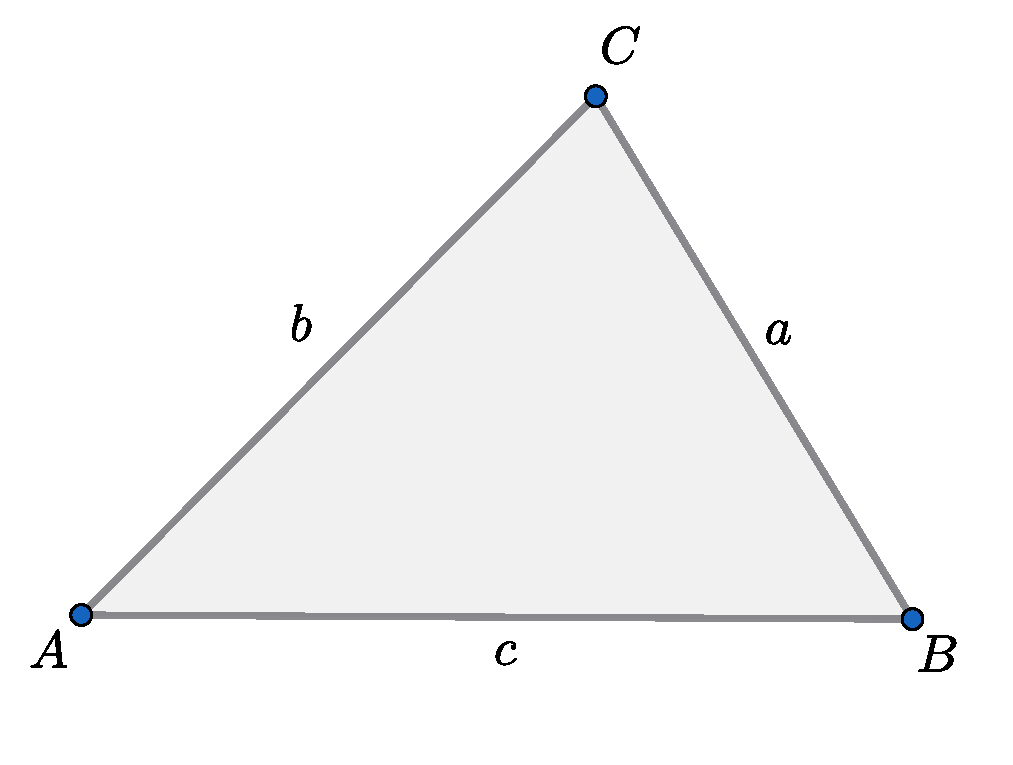
\includegraphics[scale=0.6]{25}
	\caption{}
	\label{Figure25}
\end{figure}

\newpage
\begin{theorembox}[กฎของไซน์]
กำหนดให้ $\triangle ABC$ เป็นสามเหลี่ยมใด ๆ
ซึ่งถูกล้อมรอบด้วยวงกลมรัศมี $R$
และมีความยาวด้านตรงข้ามมุม $A,B$ และ $C$
เท่ากับ $a,b$ และ $c$ ตามลำดับ ดังรูปที่~\ref{Figure26}
จะได้ความสัมพันธ์ว่า
\[
\frac{a}{\sin(A)}=\frac{b}{\sin(B)}=\frac{c}{\sin(C)}=2R
\]
\end{theorembox}

\begin{figure}[H]
	\centering
	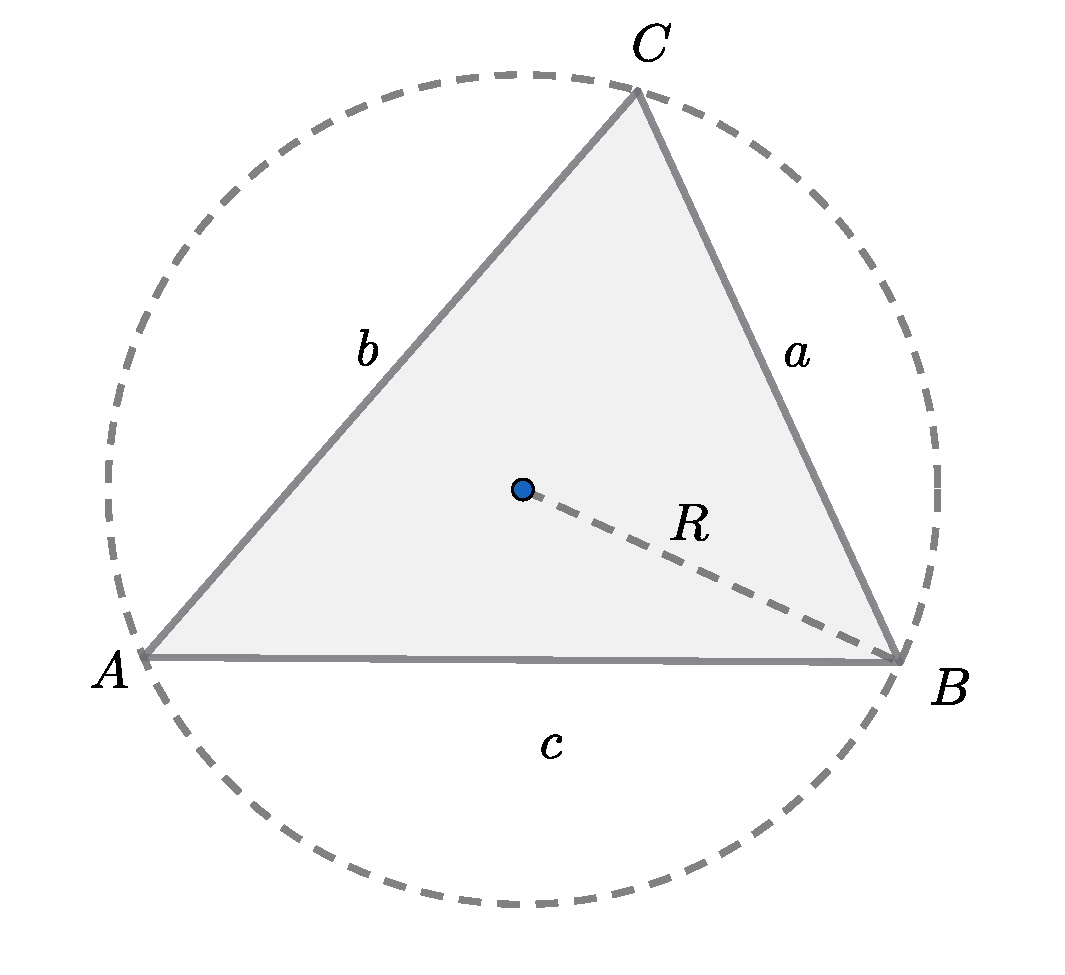
\includegraphics[scale=0.5]{26}
	\caption{}
	\label{Figure26}
\end{figure}

\begin{examplebox}[NETSAT คณิตศาสตร์ สิงหาคม 2568]  
กำหนดให้ $\triangle ABC$ มี $AB=3$ หน่วย $AC=3$ หน่วย และ $\angle A =120^{\circ}$ จงหาความยาวด้าน $BC$
\begin{multicols}{2}
\begin{enumerate}
\item $3\sqrt{3}$
\item $3\sqrt{5}$
\item $3\sqrt{7}$
\item $9$
\end{enumerate}
\end{multicols}
\end{examplebox}
\newpage
\begin{examplebox}[NETSAT คณิตศาสตร์ กุมภาพันธ์ 2565]
กำหนดให้ $\triangle A B C$ มีความยาวด้าน $BC$ คือ $a$ หน่วย มีความยาวด้าน $CA$ คือ $b$ หน่วย มีความยาวด้าน $AB$ คือ $c$ หน่วย และยังสอดคล้องกับเงื่อนไข
\[3(a+b)(a-b)=c(2 b+3 c)\]
แล้ว $\tan(A)$ มีค่าเท่าใด
\begin{multicols}{2}
\begin{enumerate}
\item $\dfrac{1}{2 \sqrt{2}}$
\item $-\dfrac{1}{2 \sqrt{2}}$
\item $2 \sqrt{2}$
\item $-2 \sqrt{2}$
\end{enumerate}
\end{multicols}
\end{examplebox}
\newpage
\begin{examplebox}[NETSAT คณิตศาสตร์ กุมภาพันธ์ 2565]
ให้ $\alpha$ และ $\beta$ เป็นค่าคงตัว ซึ่ง $0<\alpha<\beta<2\pi$ \\
กำหนดให้ฟังก์ชัน
\[f(x)=\sin^2(x)+\sin^2(x+\beta)+\sin^2(x+\beta)\,\, \text{มีค่าเป็นค่าคงตัว $c$ สำหรับ $0 \leq x \leq 2 \pi$}\]
แล้ว $c$ มีค่าเท่าไร
\begin{multicols}{2}
\begin{enumerate}
\item $0$
\item $1$
\item $\dfrac{3}{2}$
\item $2$
\end{enumerate}
\end{multicols}
\end{examplebox}
\newpage
\begin{examplebox}[NETSAT คณิตศาสตร์ 2566]
จากรูปที่~\ref{Figure27} จงหาขนาดของมุม $B$
\begin{multicols}{2}
\begin{enumerate}
\item $30^{\circ}$
\item $45^{\circ}$
\item $60^{\circ}$
\item $75^{\circ}$
\end{enumerate}
\end{multicols}
\end{examplebox} 
\begin{figure}[H]	 
	\centering
	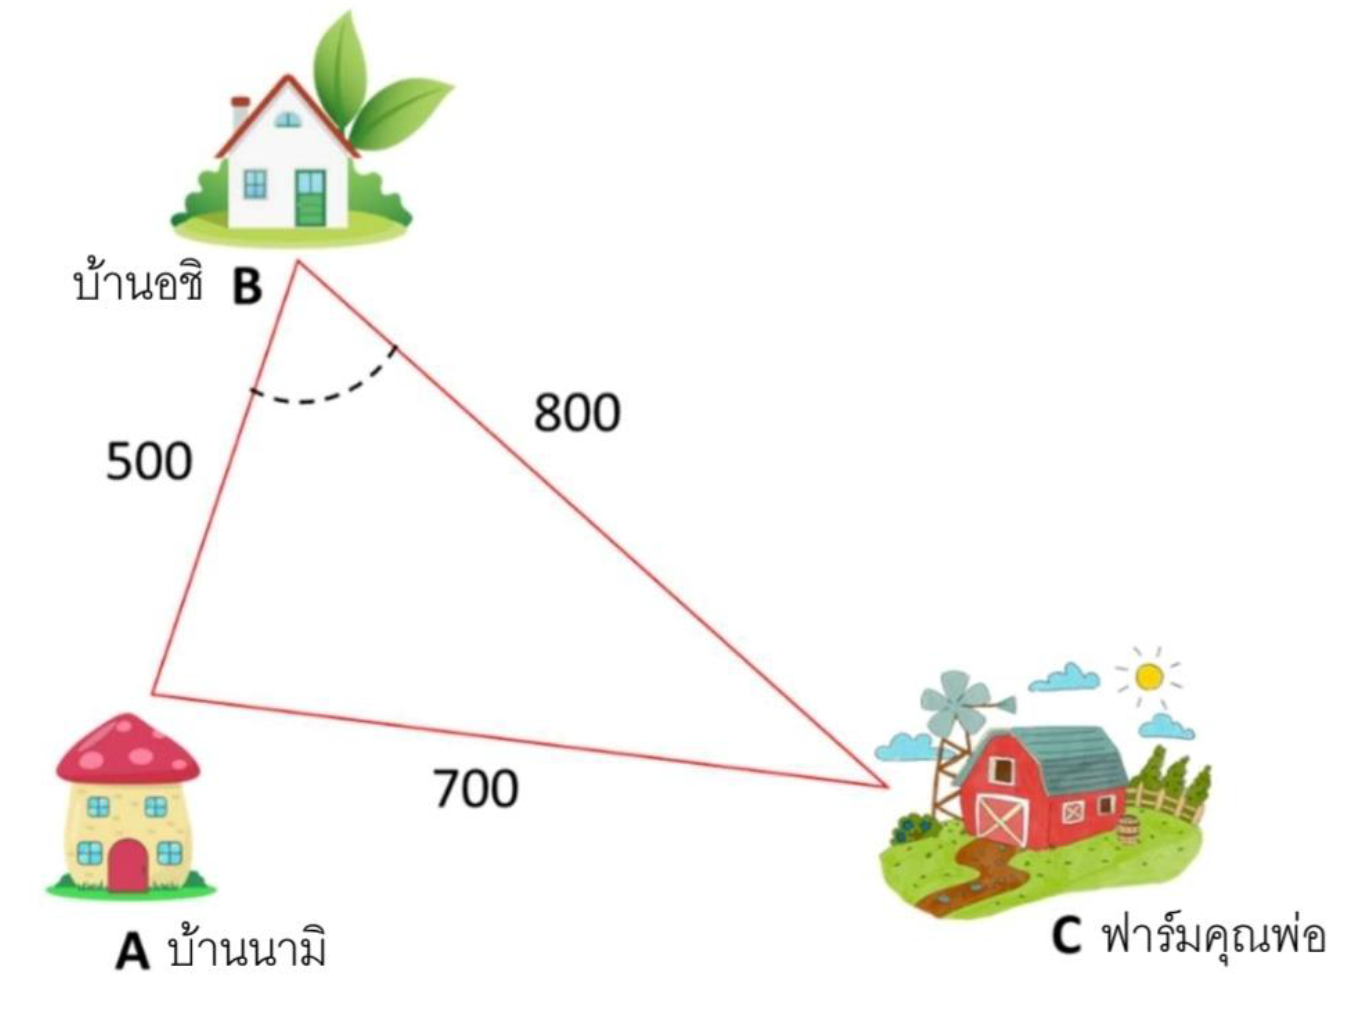
\includegraphics[scale=0.5]{27}
    	\caption{}
       \label{Figure27}
\end{figure} 
\newpage
\begin{examplebox}[NETSAT คณิตศาสตร์ 2566]
จากรูปที่~\ref{Figure27} นามิและอชินัดพบกันที่จุด $O$ ซึ่งอยู่ห่างจากบ้านของนามิ บ้านของอชิ และฟาร์มคุณพ่อ เป็นระยะเท่ากัน จงหาระยะทางโดยประมาณจากบ้านของบ้านของอชิและฟาร์มคุณพ่อไปยังจุด $O$ ที่ใกล้เคียงมากที่สุด โดยกำหนดให้ $\sqrt{3}=1.73$
\begin{multicols}{2}
\begin{enumerate}
\item $300$ เมตร
\item $400$ เมตร
\item $500$ เมตร
\item $600$ เมตร
\end{enumerate}
\end{multicols}
\end{examplebox} 
\newpage
\begin{examplebox}[NETSAT คณิตศาสตร์ 2566]
รูปที่~\ref{Figure28} แสดงภาพมุมสูงของม้าหมุนในสวนแห่งหนึ่ง โดยมีที่นั่งอยู่บนเส้นรอบวงสองวงและหมุนรอบจุดศูนย์กลาง $O$ โดยมีรัศมีของวงกลมด้านนอกเท่ากับ $10$ เมตร รัศมีของวงกลมด้านในเท่ากับ $6$ เมตร
กำหนดให้ที่นั่ง $A$ และ $B$ อยู่ข้างกันบนเส้นรอบวงด้านนอกและด้านในตามลำดับโดยไม่คำนึงขนาดของที่นั่ง เมื่อที่นั่ง $A$ และ $B$ เริ่มขยับไปพร้อมๆ กัน รูปที่ 2 แสดงให้เห็นตำแหน่ง $A$ และ $B$ หลังผ่านไป $2-3$ นาที หลังจากเริ่มหมุน ถ้า $\angle AOB=\theta$ และ $\cos(\theta)=\dfrac{11}{24}$ จงหาระยะทางจาก $A$ มา $B$
\begin{multicols}{2}
\begin{enumerate}
\item $7$
\item $9$
\item $11$
\item $13$
\end{enumerate}
\end{multicols}
\end{examplebox} 
\begin{figure}[H]	 
	\centering
	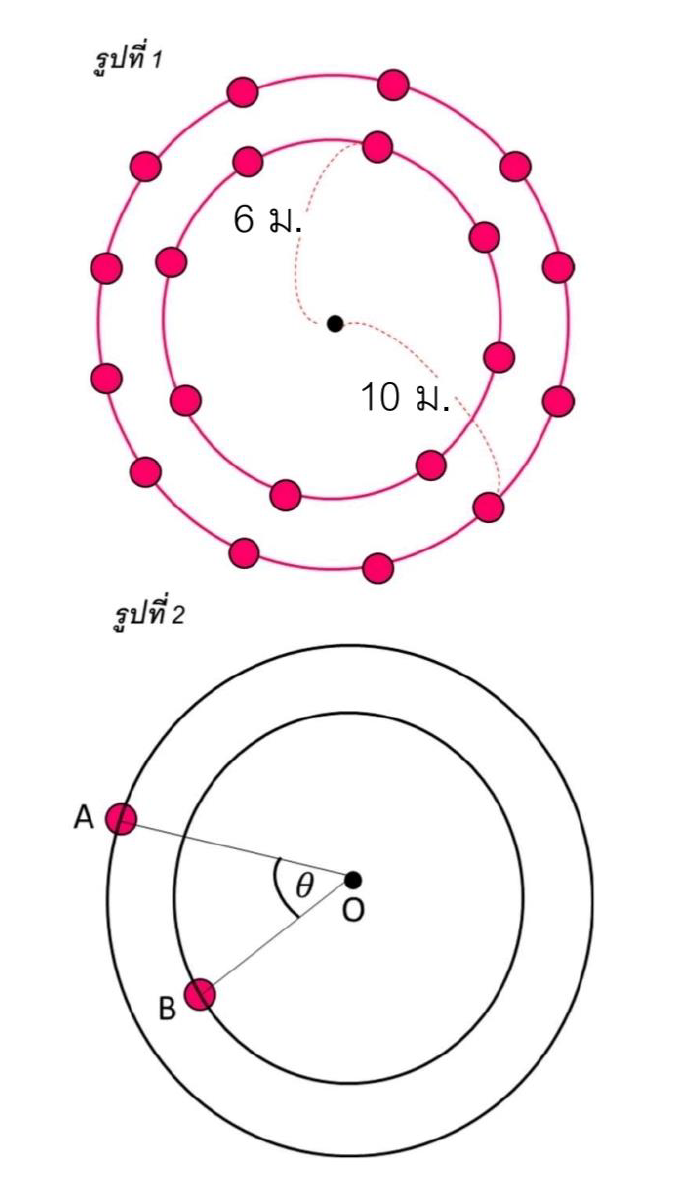
\includegraphics[scale=0.7]{28}
    	\caption{}
       \label{Figure28}
\end{figure}

\newpage
\thispagestyle{empty}
\begin{remarkbox}
วงกลมวงหนึ่งและวงเดียวเท่ากันที่สามารถผ่านจุดทั้งสามจุดที่ไม่อยู่ในแนวเส้นตรงเดียวกัน\\
จากรูปที่~\ref{Figure62} กำหนดให้จุด $A,B$ และ $C$ เป็นจุดสามจุดที่ไม่อยู่ในแนวเส้นตรงเดียวกัน จึงสามารถถูกวงกลมเพียงวงเดียวผ่านทั้งสามจุด
\end{remarkbox}

\begin{figure}[H]
	\centering
	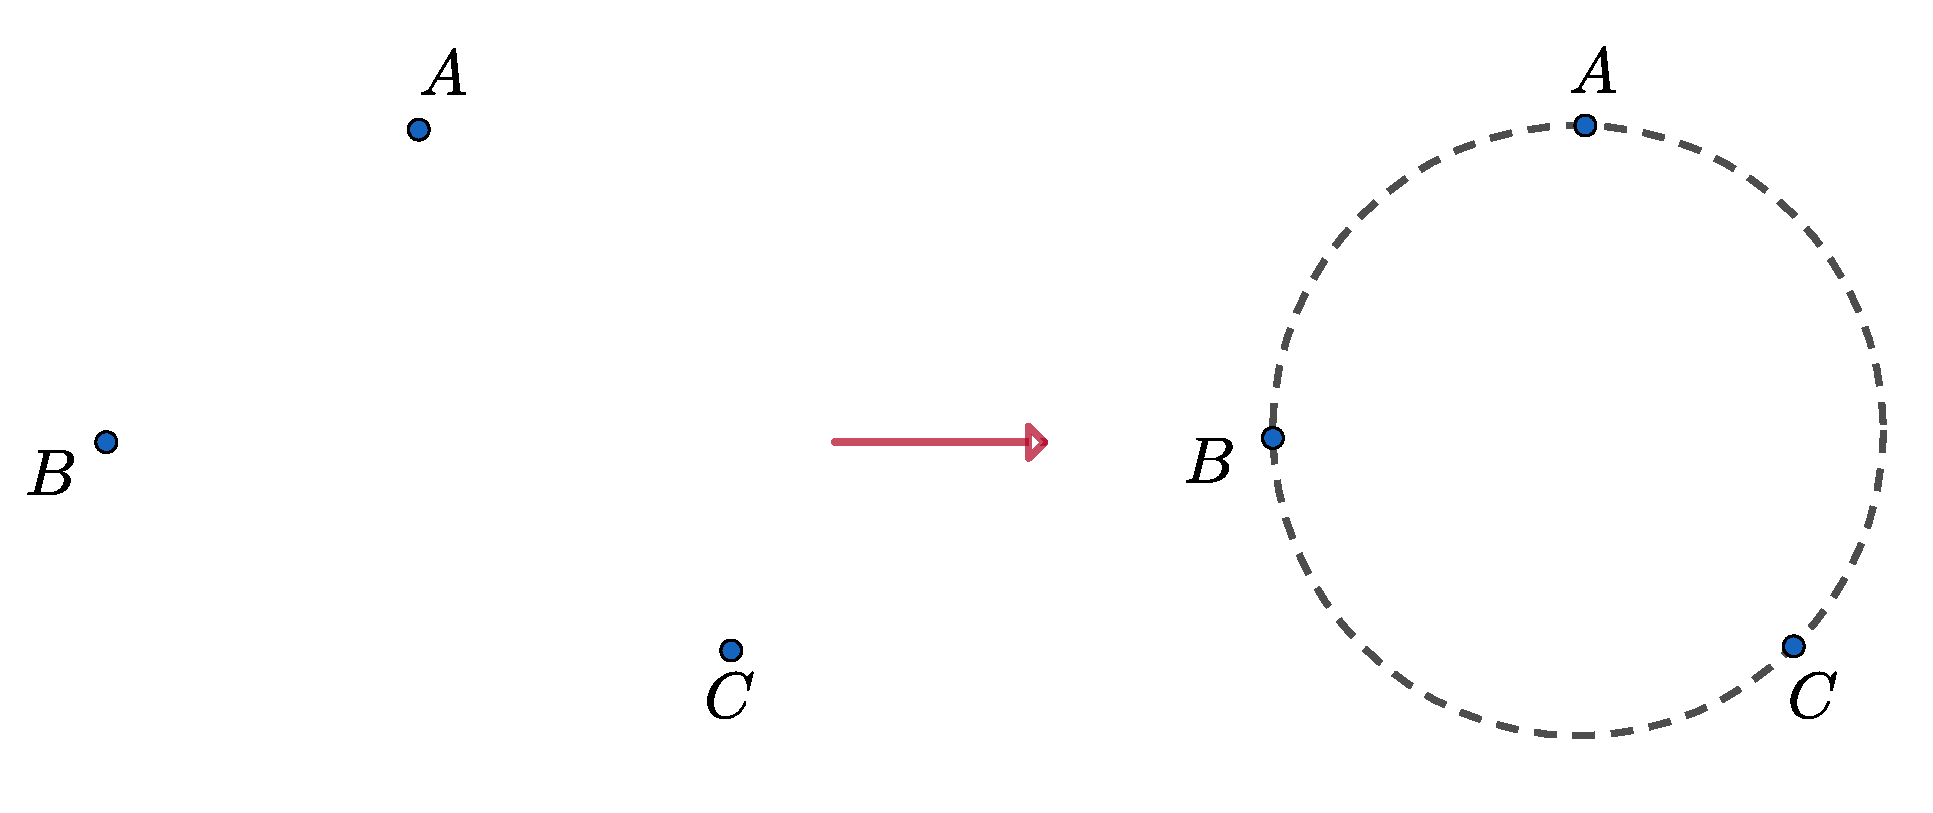
\includegraphics[scale=0.55]{62}
	\caption{}
	\label{Figure62}
\end{figure}

\begin{remarkbox}
จากจุดจุดหนึ่งภายในวงกลม ถ้าลากส่วนของเส้นตรงไปยังเส้นรอบวงให้ยาวเท่ากันได้ \textbf{มากกว่าสองเส้นขึ้นไป} แล้วจุดนั้นจะเป็นจุดศูนย์กลางของวงกลม\\
จากรูปที่~\ref{Figure63} ลากส่วนของเส้นตรงจากจุด $O$ ไปยังจุด $A,B$ และ $C$ ที่อยู่บนเส้นรอบวงได้ความยาวเท่ากัน จึงสามารถสรุปได้ว่าจุด $O$ เป็นจุดศูนย์กลางของวงกลม
\end{remarkbox}
\begin{figure}[H]
	\centering
	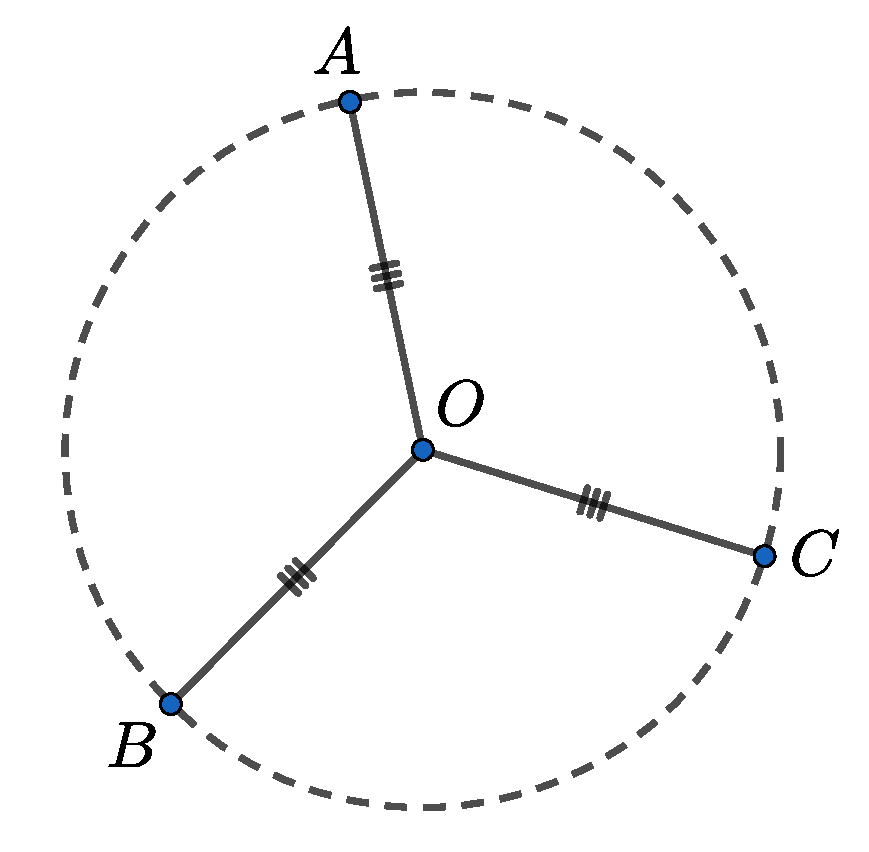
\includegraphics[scale=0.52]{63}
	\caption{}
	\label{Figure63}
\end{figure}

